\documentclass{beamer}
\usetheme{default} 

\setbeamercolor{structure}{fg=green!40!black} 
\usebackgroundtemplate{
    \centering
\includegraphics[width=\paperwidth,height=\paperheight]{images/android_wall}
}
\setbeamertemplate{navigation symbols}{}

\usepackage[utf8x]{inputenc}
\usepackage{default}
\usepackage{listings}

\lstset{language=java, basicstyle=\small, commentstyle=\color{gray}}
\lstset{frame=single}

\usefoottemplate{
  \vbox{
    \tinycolouredline{structure!25}{
      \color{black}\textbf{
        \insertshortauthor\hfill
        Android @ Szczecin 2011
      } 
    }
%    \tinycolouredline{structure}{
%      \color{white}\textbf{\insertshorttitle}\hfill
%    } 
  }
}

\title{Android @ Szczecin \\ 2011}
\author{Konrad Malawski \\ konrad.malawski@java.pl}

\begin{document}

\begin{frame}
\titlepage
\end{frame}

\begin{frame}
 \frametitle{me.about();}
 \centering
 Konrad Malawski \\
 Lunar Logic Polska \\
 _\\
 PolishJUG \\ 
 GeeCON\\
 KrakówGTUG\\
 _\\
 twitter: @ktosopl\\
 github: ktoso\\
 blog: blog.project13.pl\\
\end{frame}

\begin{frame}
\frametitle{Architektura}

  \begin{figure}[t]
    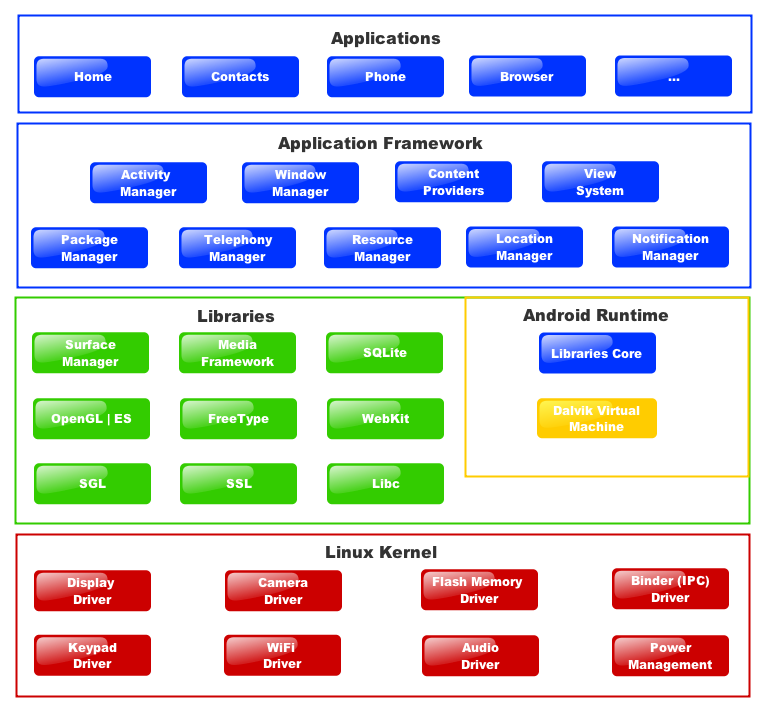
\includegraphics[height=0.62\textheight,keepaspectratio=true,clip=true]{images/platform}
    \caption{Architektura systemu Android}
  \end{figure}

\end{frame}

\begin{frame}
 \frametitle{Słowa na dziś}
 \begin{itemize}
  \item \textbf{Activity}
  \item \textbf{Service}
  \item \textbf{Intent}
  \item 
  \item 
  \item \_\_\_\_\_\_\_\textbf{Manager}
 \end{itemize}

\end{frame}

\begin{frame}
  \frametitle{Przykłady Managerów}
      \begin{itemize}
        \item \textbf{NotificationManager} - dla powiadomień
        \item \textbf{AccountManager} - dla kont użytkownika, np. konto skype / gmail (system-wide)
        \item \textbf{AlarmManager} - dla alarmów
        \item \textbf{BatteryManager} - stan baterii
        \item \textbf{ClipboardManager} - schowek nie jest taki trywialny, ma całe własne API
        \item \textbf{ConnectivityManager} - możemy sprawdzić czy Internet jest dostępny. Via 3G czy WiFi?
        \item \textbf{LocationManager} - dostęp do pozycji (również GPS)
        \item nowe: \textbf{FragmentManager} - nowe api do umieszczania wiele activity na jednym ekranie (upraszczając)
        \item nowe: \textbf{DownloadManager} - zaawansowany menadżer pobierania plików w tle (w \textbf{Honeycomb})
      \end{itemize}
\end{frame}



\begin{frame}
 \begin{figure}[ct]
  \centering
  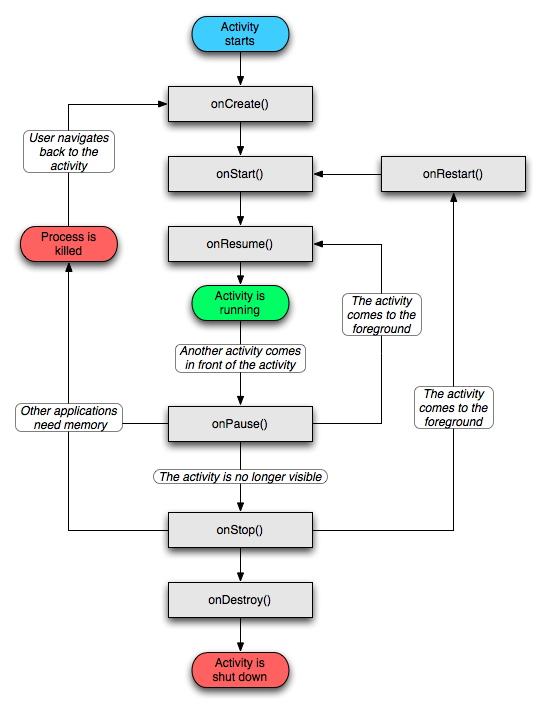
\includegraphics[height=\textheight]{images/activity_lifecycle}
 \end{figure}

\end{frame}

\begin{frame}[fragile]
\frametitle{Activity}
\begin{lstlisting}
  public class MainActivity extends Activity {
    public void onCreate(Bundle savedState) {
      /**/
    }
  }
\end{lstlisting}

\end{frame}

\begin{frame}
 todo, informacje o service i opis lifecycle
\end{frame}

% UI STUFF
\begin{frame}[fragile]
 \frametitle{Pyszne tosty z masełkiem (android.widget.Toast)}

\begin{figure}[h]
 \centering
 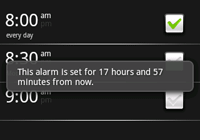
\includegraphics[height=0.40\textheight,keepaspectratio=true]{images/toast}
\end{figure}


 Przykład użycia: 
 \begin{lstlisting}
Toast.makeText(getApplicationContext(),
               "Halo Szczecin!", 
               Toast.LENGTH_LONG)
     .show();
 \end{lstlisting}

\end{frame}

\begin{frame}[fragile]
\frametitle{Co więcej potrafi Toast?}
\begin{lstlisting}
 Toast t = Toast.makeText(this, txt, LENGTH_SHORT);
\end{lstlisting}

\pause

Można mu zmienić pozycję:
\begin{lstlisting}
t.setGravity(Gravity.TOP|Gravity.LEFT, 0, 0);
\end{lstlisting}

\pause

lub podmienić widok:
\begin{lstlisting}
View customView = findViewById(R.id.custom_view);
/**/
t.setView(customView)
 \end{lstlisting}

\end{frame}


% ------------------------------ MAPS ------------------------------ 
\begin{frame}
\frametitle{Google Maps}

\begin{figure}[tc]
  \centering
  
\includegraphics[height=0.45\textheight,keepaspectratio=true]{images/maps_icon}
\end{figure}

Istnieje pewien ''problem'' z Google Maps oraz niektórymi innymi API. \\
\textbf{Nie są one dostępne bez odpowiedniego klucza oraz podpisania swojej aplikacji!}
\end{frame}

\begin{frame}
 \frametitle{MapsAPI key sign-up}
  \centering Rejestrujemy są po klucz na: \\
  \centering http://code.google.com/intl/pl-PL/android/maps-api-signup.html \\
  _\\
  \centering BitLy: \textbf{http://bit.ly/mapsapiandroid}\\
\end{frame}

\begin{frame}[fragile]
 \frametitle{Permissions}

W naszym przypadku interesują nas:

\begin{itemize}
 \item \verb|android.permission.ACCESS_COARSE_LOCATION|
 \item \verb|android.permission.ACCESS_FINE_LOCATION|
\end{itemize}

\pause

oraz INTERNET, skoro chcemy wyświetlić mapkę:
\begin{itemize}
 \item \verb|android.permission.INTERNET|
\end{itemize}

\end{frame}



\begin{frame}[fragile]
 \frametitle{Zdobywanie MD5 klucza 'debug'}
\begin{lstlisting}
 keytool -list -alias androiddebugkey \
-keystore <path_to_debug_keystore>.keystore \
-storepass android -keypass android
\end{lstlisting}
\end{frame}


\begin{frame}[fragile]
\frametitle{Zdobywanie Md5 klucza 'release'}

\textbf{keytool -list -keystore ~/android.keystore }

\begin{lstlisting}
Keystore type: JKS
Keystore provider: SUN

Your keystore contains 1 entry
android-key, Jul 3, 2011, PrivateKeyEntry, 
Certificate fingerprint (MD5): AA:AA:AA:AA...
\end{lstlisting}

\end{frame}


\end{document}
